\documentclass{article}
\usepackage{tikz}

\begin{document}

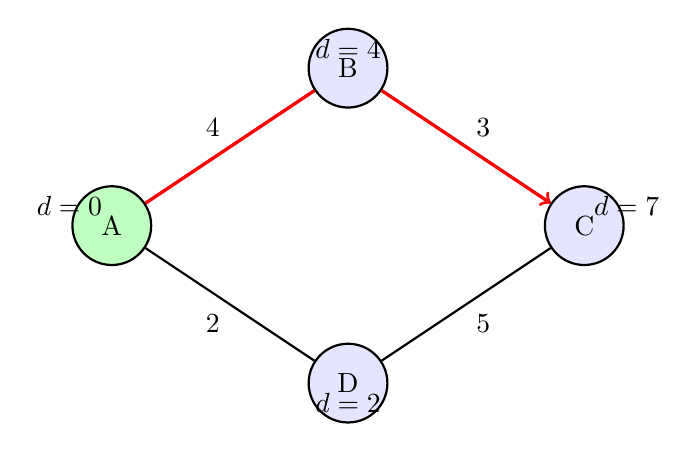
\begin{tikzpicture}[
    vertex/.style={
        circle,
        draw,
        thick,
        minimum size=10mm
    }
]

\node[vertex, fill=green!25] (A) at (0,2) {A};
\node[vertex, fill=blue!10] (B) at (3,4) {B};
\node[vertex, fill=blue!10] (C) at (6,2) {C};
\node[vertex, fill=blue!10] (D) at (3,0) {D};

\draw[thick] (A) -- node[above left] {4} (B);
\draw[thick] (B) -- node[above right] {3} (C);
\draw[thick] (A) -- node[below left] {2} (D);
\draw[thick] (D) -- node[below right] {5} (C);

% Highlight shortest path
\draw[very thick, red, ->] (A) -- (B) -- (C);

% Distance labels
\node[above left] at (A) {$d=0$};
\node[above] at (B) {$d=4$};
\node[above right] at (C) {$d=7$};
\node[below] at (D) {$d=2$};

\end{tikzpicture}

\end{document}
